\documentclass[tikz]{standalone}
\usetikzlibrary{graphs, graphs.standard}

\begin{document}
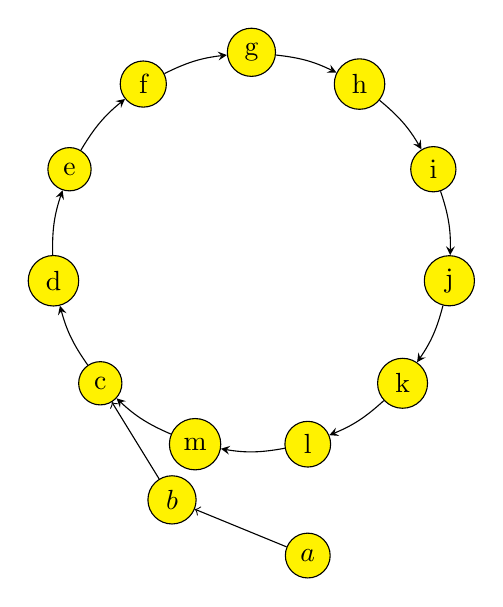
\begin{tikzpicture}

    \tikzstyle{every node}=[draw,shape=circle,fill=yellow];

    \graph[nodes={draw, circle}, clockwise, radius=1in, nodes, n=11, V={g,...,m,c,d,e,f}, ->, edge={bend left=10,>=stealth}]{subgraph C_n[name=outer]};

    \node (b)[below right of=outer c][left of=outer m]{$b$};
    \node (a)[below right of=b][below left of=outer l]{$a$};

    \draw[->](a) -- (b);
    \draw[->](b) -- (outer c);

\end{tikzpicture}
\end{document}
